\documentclass[tikz,border=3pt]{standalone}
\usepackage{amsmath,amssymb}
\usetikzlibrary{arrows.meta,calc}
\definecolor{curveblue}{HTML}{245C86}
\definecolor{accent}{HTML}{A65E2E}
\definecolor{curveteal}{HTML}{287B6D}
\definecolor{curveviolet}{HTML}{76578B}
\begin{document}
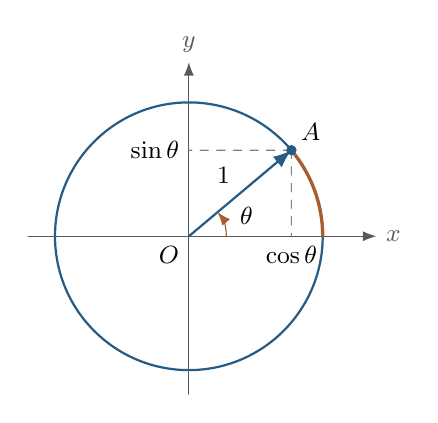
\begin{tikzpicture}[font=\small,>=Latex,line cap=round,line join=round]

\begin{scope}[scale=1.7]
\draw[curveblue,thick] (0,0) circle (1);
\draw[accent,very thick] (1,0) arc[start angle=0,end angle=40,radius=1];
\draw[->,black!65] (-1.2,0)--(1.4,0) node[right]{$x$};
\draw[->,black!65] (0,-1.18)--(0,1.3) node[above]{$y$};
\coordinate (A) at ({cos(40)},{sin(40)});
\draw[black!50,dashed] (A)--({cos(40)},0) (A)--(0,{sin(40)});
\draw[->,curveblue,thick] (0,0)--(A);
\draw[accent,->] (.28,0) arc[start angle=0,end angle=40,radius=.28];
\node at (.43,.15) {$\theta$};
\node[above left] at (.38,.32) {$1$};
\node[below] at ({cos(40)},0) {$\cos\theta$};
\node[left] at (0,{sin(40)}) {$\sin\theta$};
\node[below left] at (0,0) {$O$};
\node[above right] at (A) {$A$};
\fill[curveblue] (A) circle (1.1pt);
\end{scope}
\end{tikzpicture}
\end{document}
